\documentclass{article}

\usepackage{fancyhdr}
\usepackage{extramarks}
\usepackage{amsmath}
\usepackage{amsthm}
\usepackage{amsfonts}
\usepackage{tikz}
\usepackage[plain]{algorithm}
\usepackage{algpseudocode}
\usepackage[shortlabels]{enumitem}
\usepackage{mathtools}
\usepackage{amssymb}
\usepackage{graphicx}

\usetikzlibrary{automata,positioning}

%
% Basic Document Settings
%

\topmargin=-0.45in
\evensidemargin=0in
\oddsidemargin=0in
\textwidth=6.5in
\textheight=9.0in
\headsep=0.25in

\linespread{1.1}

\pagestyle{fancy}
\lhead{\hmwkAuthorName}
\chead{\hmwkClass\ (\hmwkClassInstructor\ \hmwkClassTime): \hmwkTitle}
\lfoot{\lastxmark}
\cfoot{\thepage}

\renewcommand\headrulewidth{0.4pt}
\renewcommand\footrulewidth{0.4pt}

\setlength\parindent{0pt}

%
% Create Problem Sections
%

\newcommand{\enterProblemHeader}[1]{
    \nobreak\extramarks{}{Problem \arabic{#1} continued on next page\ldots}\nobreak{}
    \nobreak\extramarks{Problem \arabic{#1} (continued)}{Problem \arabic{#1} continued on next page\ldots}\nobreak{}
}

\newcommand{\exitProblemHeader}[1]{
    \nobreak\extramarks{Problem \arabic{#1} (continued)}{Problem \arabic{#1} continued on next page\ldots}\nobreak{}
    \stepcounter{#1}
    \nobreak\extramarks{Problem \arabic{#1}}{}\nobreak{}
}

\setcounter{secnumdepth}{0}
\newcounter{partCounter}
\newcounter{homeworkProblemCounter}
\setcounter{homeworkProblemCounter}{1}
\nobreak\extramarks{Problem \arabic{homeworkProblemCounter}}{}\nobreak{}

%
% Homework Problem Environment
%
% This environment takes an optional argument. When given, it will adjust the
% problem counter. This is useful for when the problems given for your
% assignment aren't sequential. See the last 3 problems of this template for an
% example.
%
\newenvironment{homeworkProblem}[1][-1]{
    \ifnum#1>0
        \setcounter{homeworkProblemCounter}{#1}
    \fi
    \section{Problem \arabic{homeworkProblemCounter}}
    \setcounter{partCounter}{1}
    \enterProblemHeader{homeworkProblemCounter}
}{
    \exitProblemHeader{homeworkProblemCounter}
}

\newcommand{\hmwkTitle}{Homework 4}
\newcommand{\hmwkDueDate}{October 5, 2023}
\newcommand{\hmwkClass}{Discrete Math}
\newcommand{\hmwkClassTime}{Section 003}
\newcommand{\hmwkClassInstructor}{Reese Lance}
\newcommand{\hmwkAuthorName}{\textbf{Rushil Umaretiya}}

%
% Title Page
%

\title{
    \vspace{2in}
    \textmd{\textbf{\hmwkClass:\ \hmwkTitle}}\\
    \normalsize\vspace{0.1in}\small{\textbf{Due\ on\ \hmwkDueDate\ at 11:59pm}}\\
    \normalsize\text{Tuesday/Thursday 11:00-12:15, Phillips 383}\\
    \vspace{0.1in}\large{\textit{\hmwkClassInstructor\ - \hmwkClassTime}}
    \vspace{3in}
}

\author{\hmwkAuthorName\\\small{rumareti@unc.edu}}
\date{}

\renewcommand{\part}[1]{\textbf{\large Part \Alph{partCounter}}\stepcounter{partCounter}\\}

%
% Various Helper Commands
%

% Useful for algorithms
\newcommand{\alg}[1]{\textsc{\bfseries \footnotesize #1}}

% For derivatives
\newcommand{\deriv}[1]{\frac{\mathrm{d}}{\mathrm{d}x} (#1)}

% For partial derivatives
\newcommand{\pderiv}[2]{\frac{\partial}{\partial #1} (#2)}

% Integral dx
\newcommand{\dx}{\mathrm{d}x}

% Alias for the Solution section header
\newcommand{\solution}{\textbf{\large Solution}}

\newcommand{\unit}[1]{\section{Unit #1}}
\newcommand{\problem}[1]{\textbf{\##1}}
\newcommand{\prob}[1]{\problem{#1}}


% Probability commands: Expectation, Variance, Covariance, Bias
\newcommand{\E}{\mathrm{E}}
\newcommand{\Var}{\mathrm{Var}}
\newcommand{\Cov}{\mathrm{Cov}}
\newcommand{\Bias}{\mathrm{Bias}}

\renewcommand{\And}{\wedge}
\newcommand{\Or}{\vee}
\newcommand{\Xor}{\oplus}
\newcommand{\Not}{\neg}
\newcommand{\Implies}{\rightarrow}
\newcommand{\Iff}{\leftrightarrow}

\newcommand{\AllIntegers}{\mathbb{Z}}
\newcommand{\AllRationals}{\mathbb{Q}}
\newcommand{\AllReals}{\mathbb{R}}
\newcommand{\AllComplexes}{\mathbb{C}}

\begin{document}

\maketitle

\pagebreak

\unit{5.1}
\prob{10}
\begin{enumerate}[a)]
    \item Find a formula for
    \begin{align*}
        \frac{1}{1\cdot2}+\frac{1}{2\cdot3}+\ldots+\frac{1}{n(n+1)}
    \end{align*}
    by examining the values of this expression for small values of \(n\).\\

Given the following equation,
\begin{align*}
    P(n) &= \sum_{i=1}^{n}\frac{1}{n(n+1)}\\
\end{align*}
We can find the following values for \(P(x)\) and generalize a formula for \(P(n)\).
\begin{align*}
    P(1) &&= \frac{1}{2}\\
    P(2) &= \frac{1}{2}+\frac{1}{6}&=\frac{2}{3}\\
    P(3) &= \frac{1}{2}+\frac{1}{6}+\frac{1}{12}&=\frac{3}{4}\\
    P(4) &= \frac{1}{2}+\frac{1}{6}+\frac{1}{12}+\frac{1}{20}&=\frac{4}{5}\\
    P(n) &&= \frac{n}{n+1}
\end{align*}
    \item Prove the formula you conjectured in part (a).
\begin{proof}
    We will prove the formula by induction.\\
    \textbf{Base Case:} \(n=1\)
    \begin{align*}
        P(1) = \frac{1}{1+1} = \frac{1}{2}
    \end{align*}
    \textbf{Inductive step:}
    Given P(n), we will prove P(n+1).
    \begin{align*}
        P(n+1) &= \sum_{i=1}^{n+1}\frac{1}{n(n+1)}\\
        &= \sum_{i=1}^{n}\frac{1}{n(n+1)}+\frac{1}{(n+1)(n+2)}\\
        &= \frac{n}{n+1}+\frac{1}{(n+1)(n+2)}\\
        &= \frac{n(n+2)+1}{(n+1)(n+2)}\\
        &= \frac{(n+1)^2}{(n+1)(n+2)}\\
        &= \frac{n+1}{n+2}
    \end{align*}
    Thus, \(P(n) \implies P(n+1)\) and \(P(n)\) is true.
\end{proof}
\end{enumerate}
\pagebreak
\prob{34}
Prove that 6 divides \(n^3 - n\) whenever \(n\) is a nonnegative integer.\\
\begin{proof}
    Given \(P(n) = \exists k \in \AllIntegers, n^3-n = 6k\), we will show that \(\forall n \in \AllIntegers^+(P(n))\) by induction.\\
    \textbf{Base Case:} \(n=0\)
    \begin{align*}
        0^3 - 0 = 6(0)
    \end{align*}
    \textbf{Inductive step:}
    Given P(n), we will prove P(n+1).
    \begin{align*}(n+1)
        (n+1)^3-(n+1) &= n^3+3n^2+3n+1-(n+1)\\
        &= n^3+3n^2+2n\\
        &= n^3-n+(3n^2+3n)\\
        &= (n^3 - n) + 3(n)(n+1)
    \end{align*}
    Since we are assuming \(P(n)\), we can affirm that \(n^3-n\) is true. Now we can show that 6 also divides the second term,
    \begin{align*}
        \exists k \in \AllIntegers, 3(n)(n+1) &= 6k\\
        n(n+1) &= 2k
    \end{align*}
    Since any odd and even integer multiplied together is even, we can affirm that 6 divides \(3(n)(n+1)\). Since we know that,
    \begin{align*}
        \forall a,b,n \in \AllIntegers,\\n|a, n|b \implies n|(a+b).
    \end{align*}
    6 must divide \((n^3 - n) + 3(n)(n+1)\). Thus \(P(n+1)\) is true.
\end{proof}

\pagebreak
\prob{64}
Use mathematical induction to prove that if \(p\) is a prime and \(p | a_1a_2 \cdots a_n\), where \(a_i\) is an integer for \(i = 1, 2, 3, \dots , n\), then \(p | a_i\) for some integer \(i\). 
\begin{align*}
    P(n) = \forall a_1, a_2, \dots, a_n \in \AllIntegers, p | a_1a_2 \cdots a_n \implies p | a_i \text{ for some } i \in \AllIntegers .\\
\end{align*}
\textbf{Base Case:} \(n=1\)
\begin{align*}
    p | a_1 \implies p | a_1
\end{align*}
\textbf{Inductive Step:} Given P(n), we will prove P(n+1).
\begin{align*}
    P(n+1) &= p|a_1a_2\cdots a_na_{n+1} \implies p|a_i \text{ for some } i \in \AllIntegers .\\
    a_k &= a_1a_2\cdots a_n\\
    &= p|a_ka_{n+1} \implies p|a_i
\end{align*}
Since we assume \(P(n)\), we know that \(p|k \implies p|a_i\). Given that \(\forall a,b,c \in \AllIntegers, a|b \implies a|bc\), we can say that \(p|a_ka_n+1 \implies p|a_i\) and shown that \(P(n) \implies P(n+1)\), thus \(P(n+1)\) is true.
\pagebreak
\unit{2.1} 
\prob{2} Use set builder notation to give a description of each of these sets.
\begin{enumerate}[a)]
    \item \{{0, 3, 6, 9, 12}\}\\
    \begin{align*}
        A = \{x \in \AllIntegers^+ | x = 3n, 0 \leq n \leq 4\}
    \end{align*}
    \item \{{-3,-2,-1, 0, 1, 2, 3}\}
    \begin{align*}
        B = \{x \in \AllIntegers | -3 \leq x \leq 3\}
    \end{align*}
    \item \(\{m,n,o,p\}\)
    \begin{align*}
        C = \{x | x \text{ is a lowercase letter in the English alphabet, alphabetically from m to p}\}
    \end{align*}
\end{enumerate}
\pagebreak
\prob{6} For each of these pairs of sets, determine whether the first is a subset of the second, the second is a subset of the first, or neither is a subset of the other.
\begin{enumerate}[a)]
    \item the set of people who speak English, the set of people who speak English with an Australian accent\\
    \begin{align*}
        \{\text{English speakers with an Australian accent}\} \subset \{\text{English speakers}\}
    \end{align*}
    The set of people who speak English with a Australian accent is a subset of all people who speak English, as every member of the subset of individuals with an Australian accent are members of the superset of all English speakers.
    \item the set of fruits, the set of citrus fruits
    The set of all citrus
    \begin{align*}
        \{\text{all citrus fruits}\} \subset \{\text{all fruits}\}
    \end{align*}
    The set of all citrus fruits is a subset of all fruits, as every member of the subset of citrus fruits are members of the superset of all fruits.
    \item the set of students studying discrete mathematics, the set of students studying data structures
    \begin{align*}
        \{\text{Students studying discrete mathematics}\} \text{ is not related to } \{\text{Students studying data structures}\}
    \end{align*}
    The set of students studying discrete mathematics is not related to the set of students studying data structures, as there is no overlap between the two sets. Neither is a subset of the other.
\end{enumerate}
\pagebreak
\prob{12} Determine whether these statements are true or false.
\begin{enumerate}[a)]
    \item \(\emptyset \in \{\emptyset\}\)
    True. The empty set is a member of the set containing the empty set.
    \item \(\emptyset \in \{\emptyset, \{\emptyset\}\}\)
    True. The empty set is a member of the set containing the empty set and the set containing the empty set.
    \item \(\{\emptyset\} \in \{\emptyset\}\)
    False. The set containing the empty set is not a member of the set containing the empty set.
    \item \(\{\emptyset\} \in \{\{\emptyset\}\}\) True. The set containing the empty set is a member of the set containing the set containing the empty set.
    \item \(\{\emptyset\} \subset \{\emptyset, \{\emptyset\}\}\) True. The set containing the empty set is a subset of the set containing the empty set and the set containing the set containing the empty set.
    \item \(\{\{\emptyset\}\} \subset \{\emptyset, \{\emptyset\}\}\) True. The set containing the set containing the empty set is a subset of the set containing the empty set and the set containing the set containing the empty set.
    \item \(\{\{\emptyset\}\} \subset \{\{\emptyset\}, \{\emptyset\}\}\) True. Both of these sets are equivalent, therefore the set containing the set containing the empty set is a subset of the set containing the set containing the empty set and the set containing the set containing the empty set.
\end{enumerate}
\pagebreak
\prob{18}
Use a Venn diagram to illustrate the relationships \(A \subset B\) and \(A \subset C\).
\graphicspath{{./images/}}
\begin{figure}[H]
    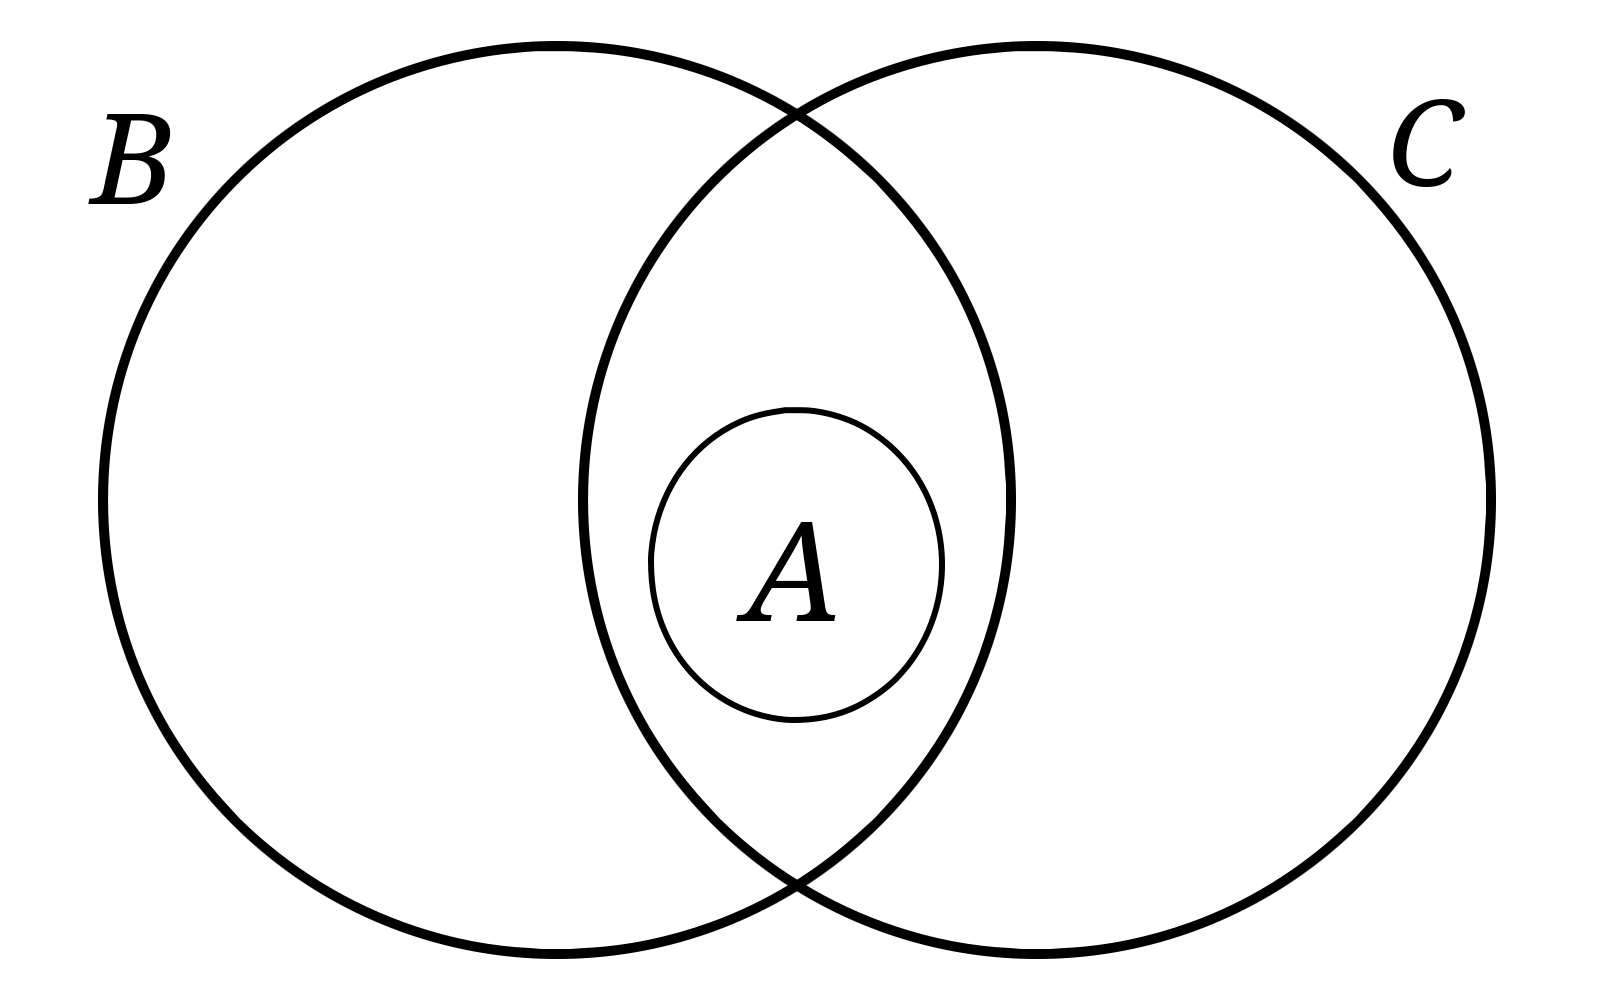
\includegraphics[width=8cm]{venn}
    \centering
\end{figure}
\pagebreak
\prob{22}
What is the cardinality of each of these sets?
\begin{enumerate}[a)]
    \item \(\emptyset\)\\
    The cardinality of the empty set is 0.
    \item \(\{\emptyset\}\)\\
    The cardinality of the set containing the empty set is 1.
    \item \(\{\emptyset, \{\emptyset\}\}\)\\
    The cardinality of the set containing the empty set and the set containing the empty set is 2.
    \item \(\{\emptyset, \{\emptyset\}, \{\emptyset, \{\emptyset\}\}\}\)\\
    The cardinality of the set contianing the empty set, set containing the empty set, and an additional set is 3.
\end{enumerate}

\pagebreak
\prob{32} Suppose that \(A \times B = \emptyset\), where \(A \text{ and } B\) are sets. What can you conclude?\\\\
Either set must be empty, as the cartesian product of two sets is the set of all ordered pairs of elements from the two sets. If the cartesian product is empty, then is no elements in at least one of the sets.

\pagebreak
\prob{44} Prove or disprove that if \(A, B, \text{and } C\) are nonempty sets and \(A \times B = A \times C\text{, then } B = C\).

The definition of the cartesian product is that \(A \times B = \{(a,b) | a \in A, b \in B\}\). If \(A \times B = A \times C\), then \(\forall a \in A, b \in B, \exists c \in C, (a,b) = (a,c)\). Since the first element of the ordered pair is the same, \(b = c\). Thus \(B = C\).\\

We can also conduct a proof by contradiction, given \(A \times B = A \times C\) we assume \(B \neq C\). We can assume that \(\exists x, x \in B, x \notin C\). We can also assume that since \(A\) is nonempty, there exists some value \(y\) in \(A\). According to the definition of the cartesian product, \((y,x) \in A \times B\). Since \(A \times B = A \times C\), \((y,x) \in A \times C\). However, since \(x \notin C\), \((y,x) \notin A \times C\). This is a contradiction, therefore \(B = C\).

\end{document}